\section{Experimental Setup}
\label{sec:experiment_setup}
Towards addressing the problems of \LossSelect{} and \SynthSelect{}, we compare the performance of iterative sound-matching experiments, where four differentiable loss functions are applied to four differentiable synthesizers. What we mean by ``performance'' is the similarity of the final output to the target, as measured by P-Loss, MSS, and---most importantly---manual listening tests.

\textbf{We hypothesize that the relative performance of loss functions for sound-matching is influenced by the method of synthesis}. If true, this would strengthen the idea that the selection of the loss function and synthesis method is not an optimization problem, but a subjective choice depending on the needs of the sound designer. 
% For clear clarity and alignment with structural norms, we recommend splitting this into three sections: (1) Experimental Setup (including synthesizer programs, loss definitions, optimization procedure); (2) Experimental Results (performance metrics, statistical tests, and rankings); and (3) Discussion (qualitative interpretation, synthesis-specific observations, and practical implications).


% We have highlighted the lack of attention given to the selection of loss functions in sound-matching, and noted that the few existing works addressing this issue evaluate their proposed losses using only simplistic sound synthesis methods. \textcolor{highlight}{We hypothesize that the best performing loss function is influenced by the synthesis techniques utilized in the synthesizer}. This hypothesis targets the issues of \LossSelect~and \SynthSelect. 

We test four different loss functions (described in Section~\ref{sec:loss_implementation}) and compare their success in sound-matching using four different synthesizers (Section~\ref{sec:programs}). We verify the success of the sound-matching process using two automatic measures of sound similarity (MSS and P-Loss) and a manual blinded hearing test conducted by two of the authors where Likert scores~\cite{jebb2021review} of 1-5 are assigned to a subset of final outputs and the corresponding targets. Details regarding the evaluation methods are described in Section~\ref{sec:evaluation_manual_auto}.

An \textit{experiment} is one iteration of sound-matching given a loss function, target sound,
and synthesizer program. When the final iteration is complete, a score is given (automatically with an algorithm or with manual listening) to an experiment that measures its success in replicating the target sound. Consider the following simplified scenario: we have two loss functions, $L_1$ and $L_2$, and a single synthesizer program $P$ with a target parameter set $\theta^*$ where the target sound is $t$, or $P(\theta^*) = t$. We run a large number (in this case, 300 for each loss function) of experiments where we randomly set the initial ($\theta_0$) and target parameters ($\theta^*$) of $P$ and run an iterative sound-matching loop for each loss function, with maximum number of iterations set to 200. When the loop is terminated, we measure the similarity of the final output sound $x$ (where $P(\theta_{199}) = x$) to $t$, or if using P-Loss we compare $\theta_{199}$ to $\theta^*$. Having 300 experiments gives us a distribution of losses to determine whether $L_1$ or $L_2$ led to better performance. This simplified example leads us to our methodology which has four loss functions, four synthesizer programs, and three different evaluation methods of scoring sound similarity.

\subsection{Loss Function Implementation Details}
\label{sec:loss_implementation}
\subsubsection{STFT Losses}
Due to their ubiquity and lower cost of gradient calculation, we use STFT as the basis of two loss functions. As discussed in Section~\ref{sec:matching_types}, the L1 or L2 distances are the most common methods of comparing different spectrograms, however, there are situations where this might lead to shortcomings. An example given by Vahidi \textit{et al.}~\cite{vahidi2023mesostructures} is two chirplets (tones that increase in pitch) starting and ending at the same frequencies. If one of these tones is slightly shifted in time, then the spectrograms will no longer overlap at any point, despite their sonic similarity (similar to the idea that a linear equation $f(x) = ax$ can never overlap with a slightly shifted version of itself, or $f(x) = ax +\epsilon$). In this example, we do not know if this is an issue of the spectrograms, or the L1 measure used for their comparison. In fields such as computer vision, Structural Similarity Index (SSIM)~\cite{wang2004imagesssim,wang2009mean} and Scale-Invariant Mean Squared Error (SIMSE)~\cite{barron2014shapessimse} have been used as alternatives that improved performance in various tasks relative to L1.

We define the \LoneSpec~and \SIMSESpec~functions as the application of L1 and SIMSE to the STFT spectrograms. The STFT spectrogram function uses 512 FFT bins, window size of 600 samples, and hop length (how many samples the window shifts) of 100 samples. The L1 and SIMSE implementations are differentiable. 

\subsubsection{JTFS Loss}
The \JTFS~loss function is the application of L1 difference to the JTFS representations of two sounds~\cite{vahidi2023mesostructures}. The code used for the JTFS transformation is the differentiable implementation of a 1-dimensional JTFS function provided by Andreux \textit{et al.}~\cite{kymatio}.

\subsubsection{Soft-DTW Loss}
We use the soft-DTW function, which is differentiable and --- depending on its parameters --- not shift-invariant~\cite{cuturi2017soft,janati2020spatio,tavenard.blog.softdtw}. The loss function \DTWEnv~is the application of the soft-DTW function to the envelope of the two sounds being compared~\cite{lyons1997understanding}. The envelope is calculated by creating the STFT spectrogram of a sound (the same process used in Section~\ref{sec:fourier_specs}) and summing the values at each timestep. 

\subsection{The Synthesizers}
\label{sec:programs}
The synthesizer programs are meant to be simple examples that test the building blocks of digital sound synthesis. Subtractive, additive, and FM/AM synthesis are three of the most common techniques in sound design~\cite{smith1991viewpoints}. In subtractive synthesis, frequencies are removed from a sound via digital filters. In additive synthesis, complex sounds are created via the linear combination of simpler sounds~\cite{lyons1997understanding,smith2007introduction}. As discussed previously, FM/AM synthesis refers to the general technique of modulating the frequency or amplitude of a waveform (the carrier) by another waveform (the modulator).

For each program, we provide the Faust code~\cite{orlarey2009faust}, which can be run in the online IDE~\footnote{\url{https://faustide.grame.fr/}}. Faust is a functional language for audio synthesis that can succinctly define signal processing chains. Following Braun's methodology~\cite{braun2024dac}, programs are first defined in Faust, then converted (or \textit{transpiled}) to differentiable Jax functions using the DawDreamer library\footnote{\url{https://github.com/DBraun/DawDreamer}}. 


% A general overview of the programs and the predefined parameter ranges is given in Table~\ref{tab:programs}.

In the following subsections, we describe the programs and their parameters in more detail, followed by the methodology in Section~\ref{sec:methodology} and results in Section~\ref{sec:results_posthoc}.



\begin{lstlisting}[caption={\BPNoise}, label={lst:program0}, language=Faust,
                  float, floatplacement=!H, xleftmargin=1em, xrightmargin=0.5em, firstnumber=0, aboveskip=0em, belowskip=-1em]
import("stdfaust.lib");
lp_cut = hslider("lp_cut",900,50,1000,1);
hp_cut = hslider("hp_cut",100,1,120,1);
process = no.noise:fi.lowpass(3,lp_cut):fi.highpass(10,hp_cut);
\end{lstlisting}

\begin{lstlisting}[caption={\AddSineSaw}, label={lst:program1},language=Faust,float,floatplacement=!H,xleftmargin=1em,xrightmargin=0.5em,firstnumber=0,aboveskip=0em, belowskip=-1em]
import("stdfaust.lib");
saw_freq = hslider("saw_freq",800,20,1000,1);
sine_freq = hslider("sine_freq",300,20,1000,1);
sineOsc(f) = +(f/ma.SR) ~ ma.frac:*(2*ma.PI) : sin;
sawOsc(f) = +(f/ma.SR) ~ ma.frac;
process = sineOsc(sine_freq)+sawOsc(saw_freq);
\end{lstlisting}

\begin{lstlisting}[caption={\AmpMod}, label={lst:program2},language=Faust,float,floatplacement=!H,xleftmargin=1em,xrightmargin=0.5em,firstnumber=0,aboveskip=0em, belowskip=-1em]
import("stdfaust.lib");
amp = hslider("amp",0.5,0,5,0.01);
modulator = hslider("modulator",0.5,0,4,0.01);
sineOsc(f) = +(f/ma.SR) ~ ma.frac:*(2*ma.PI) : sin;
process = no.noise*sineOsc(modulator)*amp;
\end{lstlisting}

\begin{lstlisting}[caption={\FMMod}, label={lst:program3},language=Faust,float,floatplacement=!H,xleftmargin=1em,xrightmargin=0.5em,firstnumber=0,aboveskip=0em, belowskip=-1em]
import("stdfaust.lib");
carrier = hslider("carrier",100,20,1000,1);
amp = hslider("amp",6,1,20,1);
sineOsc(f) = +(f/ma.SR) ~ ma.frac:*(2*ma.PI) : sin;
sawOsc(f) = +(f/ma.SR) ~ ma.frac;
process = sineOsc(amp)*sawOsc(carrier);
\end{lstlisting}

\subsubsection{\BPNoise}
\label{sec:program0}
\BPNoise{} is a bare bones example of subtractive synthesis using digital filters~\cite{smith2007introduction}. Despite the ubiquity of subtractive synthesis in practical sound design, it has rarely been tested in differentiable sound-matching. In this program, a noise signal is fed through a band-pass (BP) filter. This removes the frequencies outside the low-pass (LP) and high-pass (HP) cutoffs. The noise generator produces all frequencies with random variation over time. The LP filter removes frequencies over its threshold frequency, and the HP removes frequencies lower than its threshold~\cite{smith2007introduction}. The search parameters are the cutoff thresholds for the LP and HP filters. Listing~\ref{lst:program0} shows the Faust code for \BPNoise.

\subsubsection{\AddSineSaw}
\label{sec:program1}
\AddSineSaw{} is an additive program that combines a saw and a sine wave function. Like subtractive synthesis, additive synthesis is a common approach to sound design that has not been extensively tested as a benchmark in sound-matching. The search parameters here are the frequency of the sine and saw oscillators. Listing~\ref{lst:program1} is the Faust code for \AddSineSaw.

\subsubsection{\AmpMod}
\label{sec:program2}
\AmpMod{} involves amplitude modulation of a noise generator by an LFO with \textit{modulator} as its frequency and a global \textit{amp} value that does not change over time and applies to the entire signal. The search parameters for this program are the LFO frequency and the amp value. The amp value acts as a global volume control, and since the sounds are normalized before analysis, it is likely inconsequential to the performance. This program is meant to be a stepping stone to \FMMod, which utilizes proper AM synthesis. Listing~\ref{lst:program2} is the Faust code for \AmpMod. 

\subsubsection{\FMMod}
\label{sec:program3}
Relative to additive and subtractive synthesis, AM/FM synthesis are less common methods of sound design. Due to their frequent use in previous works, we also tested an AM synthesizer. The synthesizer program is the multiplication of a low frequency sine oscillator with frequency parameter \textit{amp}, and a saw oscillator with frequency parameter \textit{carrier}. Listing~\ref{lst:program3} is the Faust code for \FMMod. 




\subsection{Evaluation Methods}
\label{sec:evaluation_manual_auto}
The two automatic evaluation methods used here are P-Loss and MSS, as described in Section~\ref{sec:loss_funcs}. For P-Loss, the parameters are normalized between 0-1 based on the valid ranges defined in the Faust program, and the L1 distance between the normalized parameters is calculated. MSS is computed using a hop size of $100$ samples, and FFT window lengths of $(512, 1024, 2048, 4096)$. 

Automatic sound evaluation methods are often unreliable, as their alignment with the subjective judgments of human listeners is uncertain. Therefore, listening tests are conducted by randomly sampling 40 experiment results for each program and loss function pair. Two of the authors then assign blinded similarity scores to the outputs and targets using a 5-point Likert scale (1 = no similarity, 5 = near identical)~\cite{jebb2021review}. Using Spearman's rank correlation~\cite{spearman1987proof,rebekic2015pearson}, we found a very strong rate of agreement between the human listeners (see Section~\ref{sec:consistency_in_rankings}), a good indicator that the scores assigned by manual listeners can be treated as the ground truth. We then combine the ranks assigned by both authors, giving us 80 ranks per program and loss function pair. 


% Agreement between the assigned scores is measured using Spearman’s rank correlation, which provides both a correlation coefficient ($\rho$) ranging from –1 (perfect negative correlation) to 1 (perfect positive correlation), and a p-value testing the null hypothesis of no correlation~\cite{spearman1987proof,rebekic2015pearson}. Across all programs, the correlation was very strong ($\rho = 0.86$, $p < 10^{-180}$). Per-program correlations were also very strong: $\rho = 0.71$ for \BPNoise{} ($p < 10^{-25}$), $\rho = 0.64$ for \AddSineSaw{} ($p < 10^{-19}$), $\rho = 0.84$ for \AmpMod{} ($p < 10^{-43}$), and $\rho = 0.85$ for \FMMod{} ($p < 10^{-44}$). This high rate of agreement is a good indicator that the scores assigned by manual listeners can be treated as the ground truth. 

% For each program and loss function, the blind manual hearing test gives us 80 ranks, which are given by two of the authors to a set of 40 randomly selected experiment results. This gives 160 pairs of ranks per program, and 640 for all programs. We computed Spearman correlations between the two reviewers.

\subsection{Training Parameters and Gradient Calculations}
 % Previous work utilized gradient fields for analysis of the algorithm performance~\cite{vahidi2023mesostructures}. Gradient fields are not the center of our analysis, but we include them in Appendix~\ref{appendix:gradient_fields}.
 For updating the synthesizer parameters (or weights), we use RMSProp, which operates similar to stochastic gradient descent (SGD)~\cite{goodfellow2016deep}, with the caveat that the gradients of each weight are scaled by the root-mean-square of past gradients of that weight. Based on some initial test runs, we used an arbitrary fixed learning rate of 0.045 for all experiments (learning rates used in Vahidi \textit{et al.}~\cite{vahidi2023mesostructures} is unknown). The maximum number of iterations is set to 200, where, based on our observations, the parameters have either irrecoverably diverged outside the acceptable ranges, or are stuck at a local minimum. Additionally, the gradients are large, and calculated backwards sequentially through the signal processing chain. This backward calculation resembles the \textit{exploding gradients} problem in recurrent neural networks~\cite{gers2000learning}. Gradient clipping~\cite{goodfellow2016deep} is preemptively used to ensure that the  $\ell_2$ norm of all gradients does not exceed the threshold of 1. 
% \mathbf{\gamma}_i^{\text{clipped}} = \mathbf{\gamma}_i \cdot \mathcal{S}
% \]
% Where $\mathcal{S}$ is a value less than or equal to 1, depending on whether the norm of the gradients exceeds the threshold $c$.  
% \[
% \mathcal{S} = \frac{c}{\max(\|\mathbf{\gamma}\|_2, c)}
% \]


\subsection{Determining Best Performers}
 Once the programs are transpiled to differentiable synthesizers, the iterative sound-matching procedure is:
 \begin{enumerate}
    \item Initialize $\theta^*$ and $\hat{\theta}$, i.e., random generation of target and initial parameters uniformly over a predefined range
    \item Generating the output of the synthesizer with $\hat{\theta}$ (the length of the output is set to 1 second with sample-rate of 44100 Hz) 
    \item Calculating the loss between the target and output
    \item Applying gradient updates to the synthesizer parameters
    \item Repeating the second step with the updated parameters $\hat{\theta}$, until maximum number of iterations has been reached
 \end{enumerate}
 
 Figure~\ref{fig:posthoc_evaluation} is a visualized summary of how the loss functions are ranked. We have four loss functions and four synthesizer programs. The maximum number of iterations set to 200, and 300 experiments for each loss/synthesizer combination. Each synthesizer program is paired with four loss functions and 300 experiments are conducted and evaluated automatically with P-Loss and MSS, and manually with Likert scores.

For each program and loss function pair, we have three distributions that can be used to rank the loss functions. Two with 300 automatically assigned similarities (P-Loss and MSS) and one with 80 Likert scores (combining the 40 ranks assigned by each author). For consistency and statistical robustness, the distributions are upsampled to 1000 values using bootstrapping~\cite{tibshirani1993introduction}. Bootstrapping gives an estimation of the distribution for the mean performance of each experiment. $k$ (set to 1000) samples of $n$ values (set to 100\% of the values) are taken with replacement from the empirical distribution (list of 300 performance values for MSS and P-Loss or 80 for manual rankings). The mean performance is calculated for each of the $k$ samples. The $k$ estimates of the mean performance give us a bootstrapped distribution for each loss function. 

% For each program, the loss functions are ranked using the non-parametric Scott-Knott (\gls{NPSK}) test~\cite{tantithamthavorn2017mvt,tantithamthavorn2018optimization}, which ranks the loss functions from rank 1 (best, or highest distribution values) to maximum rank of 4 (worst, with lowest distribution values). NPSK may determine that multiple functions belong to the same rank, in which case the maximum rank would be less than 4. As mentioned before, lower P-Loss and MSS values indicate higher similarity, therefore (for consistency with manually assigned ranks) the reciprocal of their output is used ($x^{-1}$, if $x$ is the P-Loss or MSS value), where higher values indicate greater similarity. 


\begin{figure*}
\resizebox{\linewidth}{!}{ % Automatically scales diagram to fit page width
\begin{tikzpicture}[
    function/.style={rectangle, draw, rounded corners, minimum width=2cm, minimum height=1cm, text centered, node distance=1.5cm},
    distribution/.style={ellipse, draw, minimum width=2cm, minimum height=1cm, text centered, node distance=1.2cm},
    gaussian/.style={draw, smooth, samples=100, domain=-2.5:2.5},
    snpk/.style={rectangle, draw, rounded corners, minimum width=2.5cm, minimum height=1cm, text centered, node distance=1.5cm, fill=blue!20},
    level 1/.style={sibling distance=6cm, level distance=2cm},
    level 2/.style={sibling distance=2cm, level distance=3cm},
    mss/.style={fill=red!50, draw=black},
    ploss/.style={fill=blue!50, draw=black},
    likert/.style={fill=green!40, draw=black}
]

% Existing functions and distributions diagram
\node[function] {Synthesizer Program}
    child { node[function] {DTW\_Onset}
        child { node[distribution, mss] {MSS}
            child[grow=down, level distance=1.5cm] {
                node[draw=none] {
                    \begin{tikzpicture}[scale=0.7]
                        \draw[red] plot (\x/3, {exp(-\x*\x)});  % Red Gaussian
                    \end{tikzpicture}
                }
            }
        }
        child { node[distribution, ploss] {P-Loss}
            child[grow=down, level distance=1.5cm] {
                node[draw=none] {
                    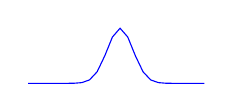
\begin{tikzpicture}[scale=0.7]
                        \draw[blue] plot (\x/3, {exp(-\x*\x)});  % Blue Gaussian
                    \end{tikzpicture}
                }
            }
        }
        child { node[distribution, likert] {Likert}
            child[grow=down, level distance=1.5cm] {
                node[draw=none] {
                    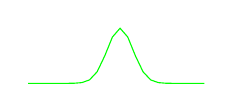
\begin{tikzpicture}[scale=0.7]
                        \draw[green] plot (\x/3, {exp(-\x*\x)});  % Green Gaussian
                    \end{tikzpicture}
                }
            }
        }
    }
    child { node[function] {L1\_Spec}
        child { node[distribution, mss] {MSS} }
        child { node[distribution, ploss] {P-Loss} }
        child { node[distribution, likert] {Likert} }
    }
    child { node[function] {SIMSE\_Spec}
        child { node[distribution, mss] {MSS} }
        child { node[distribution, ploss] {P-Loss} }
        child { node[distribution, likert] {Likert} }
    }
    child { node[function] {JTFS}
        child { node[distribution, mss] {MSS}
            child[grow=down, level distance=1.5cm] {
                node[draw=none] {
                    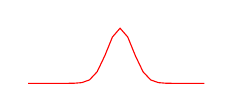
\begin{tikzpicture}[scale=0.7]
                        \draw[red] plot (\x/3, {exp(-\x*\x)});  % Red Gaussian
                    \end{tikzpicture}
                }
            }
        }
        child { node[distribution, ploss] {P-Loss}
            child[grow=down, level distance=1.5cm] {
                node[draw=none] {
                    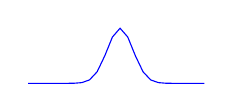
\begin{tikzpicture}[scale=0.7]
                        \draw[blue] plot (\x/3, {exp(-\x*\x)});  % Blue Gaussian
                    \end{tikzpicture}
                }
            }
        }
        child { node[distribution, likert] {Likert}
            child[grow=down, level distance=1.5cm] {
                node[draw=none] {
                    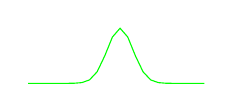
\begin{tikzpicture}[scale=0.7]
                        \draw[green] plot (\x/3, {exp(-\x*\x)});  % Green Gaussian
                    \end{tikzpicture}
                }
            }
        }
    };

% Label for the second row (Distributions)
\node at (0,-6.5) {\textbf{$\longleftarrow$\ \ \large Bootstrapped Distributions\ \ $\longrightarrow$}};

% Left side: SNPK with MSS
\node[snpk, text height=5ex, align=center, fill=red!30, draw=black] at (-6,-9) {SNPK with 4 \\ MSS distributions};
\draw[->] (-6,-9.5) -- (-6,-10.5) node[below, below] {\textbf{Ranks 1-4}};
\draw[red!40, thick] (-4.5, -8.4) -- (-2.75, -7.75);  % Line 1
\draw[red!40, thick] (-5.25, -8.4) -- (-3.5, -7.75);  % Line 2
\draw[red!40, thick] (-5.75, -8.4) -- (-5.5, -7.75);  % Line 3
\draw[red!40, thick] (-6.25, -8.4) -- (-9, -7.75);  % Line 4

% Middle: SNPK with P-Loss
\node[snpk, text height=5ex, align=center, fill=blue!40, draw=black] at (0,-9) {SNPK with 4 \\ P-Loss distributions};
\draw[->] (0,-9.5) -- (0,-10.5) node[below, below] {\textbf{Ranks 1-4}};
\draw[blue!40, thick] (1.5, -8.4) -- (3.25, -7.75);  % Line 1
\draw[blue!40, thick] (0.75, -8.4) -- (1.5, -7.75);  % Line 2
\draw[blue!40, thick] (-0.25, -8.4) -- (-1, -7.75);  % Line 3
\draw[blue!40, thick] (-0.75, -8.4) -- (-3, -7.75);  % Line 4

% Right side: SNPK with Likert
\node[snpk, text height=5ex, align=center, fill=green!30, draw=black] at (6,-9) {SNPK with 4 \\ Likert distributions};
\draw[->] (6,-9.5) -- (6,-10.5) node[below, below] {\textbf{Ranks 1-4}};
\draw[green!50, thick] (7.5, -8.4) -- (8.75, -7.75);  % Line 1
\draw[green!50, thick] (6.75, -8.4) -- (6, -7.75);    % Line 2
\draw[green!50, thick] (6.25, -8.4) -- (4, -7.75);   % Line 3
\draw[green!50, thick] (5.75, -8.4) -- (3, -7.75);     % Line 4

\end{tikzpicture}
}
\caption{For each synthesizer program, we assign ranks to the four loss functions  (\DTWEnv, \LoneSpec, \SIMSESpec, \JTFS) in three different ways, using MSS, P-Loss, or manually assigned Likert scores.}
\label{fig:posthoc_evaluation}
\end{figure*}


\section{Post hoc Analysis of Loss Performance}
\label{sec:results_posthoc}
As discussed in the previous section and summarized in Figure~\ref{fig:posthoc_evaluation}, for each program and evaluation (or scoring) method, there are four sets of 1000 bootstrapped values corresponding to the four loss functions. A post-hoc test is conducted in two stages in order to determine whether there is a difference in performance between loss functions for each program, and if so, which are the best performers. The first stage determines whether there is a difference in group means, with the null hypothesis being that all groups have similar mean ranks. The second stage ranks the loss functions from best to worst using the non-parametric Scott-Knott test (\gls{NPSK})~\cite{tantithamthavorn2017mvt,tantithamthavorn2018optimization}.
The Kruskal-Wallis test is used for the first stage~\cite{kruskal1952use}; this test pools and ranks all evaluation measures for a program, then tests whether the differences in mean rank for all loss function groups is zero. The Kruskal-Wallis test calculates an H statistic that is compared to a chi-square distribution with k-1 degrees of freedom (k is the number of groups, or 4, and degrees of freedom is 3). Using the significance level of 0.05, if the H statistic is greater than the critical value of the chi-square distribution then the null hypothesis is rejected, meaning that at least one group has a mean rank significantly above others~\cite{kruskal1952use}. Table~\ref{tab:kruskal_auto} shows the Kruskal-Wallis results for every program and evaluation method, and shows that significant differences between loss function performance measures (i.e., the bootstrapped distributions of the evaluation for each loss function) exist in all cases except MSS for the \AmpMod{} program. 

\begin{table}[ht]
\centering
\caption{Do loss functions have different median performance? Kruskal-Wallis results by program and bootstrapped evaluation results.}
\begin{tabular}{|c|c|c|c|c|}
\hline
\textbf{Program} & \textbf{Eval. Method} & \textbf{H-Stat.} & \textbf{P-value} & \textbf{Reject} \\
\hline
\BPNoise & MSS      & 81.19  & $1.70 \times 10^{-17}$ & Yes \\
\BPNoise & P-Loss  & 163.60 & $3.07 \times 10^{-35}$ & Yes \\
\BPNoise & Manual & 9.45  & $2.39 \times 10^{-2}$ & Yes \\
\AddSineSaw & MSS      & 308.97 & $1.14 \times 10^{-66}$ & Yes \\
\AddSineSaw & P-Loss  & 348.42 & $3.28 \times 10^{-75}$ & Yes \\
\AddSineSaw & Manual & 9.45  & $2.39 \times 10^{-2}$ & Yes \\
\AmpMod & MSS      & 1.35   & $0.7171$               & No \\
\AmpMod & P-Loss  & 366.76 & $3.50 \times 10^{-79}$ & Yes \\
\AmpMod & Manual & 32.71 & $3.70 \times 10^{-7}$ & Yes \\
\FMMod & MSS      & 564.65 & $4.65 \times 10^{-122}$ & Yes \\
\FMMod & P-Loss  & 229.19 & $2.07 \times 10^{-49}$ & Yes \\
\FMMod & Manual &  207.58 & $9.69 \times 10^{-45}$ & Yes \\
\hline
\end{tabular}
\label{tab:kruskal_auto}
\end{table}

% \begin{table}[ht]
% \centering
% \begin{tabular}{|c|c|c|c|}
% \hline
% \textbf{Program} & \textbf{H-Stat.} & \textbf{P-value} & \textbf{Reject} \\
% \hline
% \BPNoise & 9.45  & $2.39 \times 10^{-2}$ & Yes \\
% \AddSineSaw & 9.45  & $2.39 \times 10^{-2}$ & Yes \\
% \AmpMod & 32.71 & $3.70 \times 10^{-7}$ & Yes \\
% \FMMod & 207.58 & $9.69 \times 10^{-45}$ & Yes \\
% \hline
% \end{tabular}
% \caption{Manual ranking Kruskal-Wallis results. Significant differences are observed for all programs.}
% \label{tab:kruskal_manual}
% \end{table}



\subsection{Best Performers For Each Program}
Based on the bootstrapped distribution of scores, the NPSK algorithm ranks the loss functions from 1 (best) to a maximum of 4 (worst). In cases where the distributions are similar, multiple loss functions can be clustered into the same rank. In Figure~\ref{fig:npsk_all}, we use color-coded violin plots to visualize the best performers for each program. The corresponding colors for each rank are
\colorbox{rank1}{\textcolor{black}{\textbf{1}}} \colorbox{rank2}{\textcolor{white}{\textbf{2}}} \colorbox{rank3}{\textcolor{white}{\textbf{3}}} \colorbox{rank4}{\textcolor{black}{\textcolor{white}{\textbf{4}}}}.

\noindent\textit{Ranks that differ from the hearing test are marked with an asterisk.}

\begin{table}[htbp]
\centering
\begin{minipage}{0.45\textwidth}
    \centering
    \begin{tabular}{|c|c|c|c|}
    \hline
    \textbf{Function} & \textbf{MSS} & \textbf{P-LOSS} & \textbf{Hearing} \\
    \hline
    \textbf{SIMSE} & 1\phantom{*} & 2* & 1\phantom{*} \\
    \textbf{L1}    & 2\phantom{*} & 1* & 2\phantom{*} \\
    \textbf{JTFS}  & 3\phantom{*} & 4* & 3\phantom{*} \\
    \textbf{DTW}   & 4*           & 3\phantom{*} & 3\phantom{*} \\
    \hline
    \end{tabular}
    \caption{\footnotesize \BPNoise~ranks}
    \label{tab:p0}
\end{minipage}%
\hspace{1cm}
\begin{minipage}{0.45\textwidth}
    \centering
    \begin{tabular}{|c|c|c|c|}
    \hline
    \textbf{Function}& \textbf{MSS} & \textbf{P-LOSS} & \textbf{Hearing} \\
    \hline
    \textbf{SIMSE} & 4\phantom{*} & 4\phantom{*} & 4\phantom{*} \\
    \textbf{L1} & 2\phantom{*} & 2\phantom{*} & 2\phantom{*} \\
    \textbf{JTFS} & 1\phantom{*} & 1\phantom{*} & 1\phantom{*} \\
    \textbf{DTW} & 3\phantom{*} & 3\phantom{*} & 3\phantom{*} \\
    \hline
    \end{tabular}
    \caption{\footnotesize \AddSineSaw~ranks}
    \label{tab:p1}
\end{minipage}

\vspace{0.5cm} % Adds vertical space between rows of tables

\begin{minipage}{0.45\textwidth}
    \centering
    \begin{tabular}{|c|c|c|c|}
    \hline
    \textbf{Function} & \textbf{MSS} & \textbf{P-LOSS} & \textbf{Hearing} \\
    \hline
    \textbf{SIMSE} & 3* & 4\phantom{*} & 4\phantom{*} \\
    \textbf{L1}    & 2\phantom{*} & 2\phantom{*} & 2\phantom{*} \\
    \textbf{JTFS}  & 4* & 3\phantom{*} & 3\phantom{*} \\
    \textbf{DTW}   & 1\phantom{*} & 1\phantom{*} & 1\phantom{*} \\
    \hline
    \end{tabular}
    \caption{\footnotesize \AmpMod~ranks}
    \label{tab:p2}
\end{minipage}%
\hspace{1cm}
\begin{minipage}{0.45\textwidth}
    \centering
    \begin{tabular}{|c|c|c|c|}
    \hline
    \textbf{Function} & \textbf{MSS} & \textbf{P-LOSS} & \textbf{Hearing} \\
    \hline
   \textbf{SIMSE} & 2\phantom{*} & 2\phantom{*} & 2\phantom{*} \\
    \textbf{L1} & 3\phantom{*} & 3\phantom{*} & 3\phantom{*} \\
    \textbf{JTFS} & 4\phantom{*} & 4\phantom{*} & 4\phantom{*} \\
    \textbf{DTW} & 1\phantom{*} & 1\phantom{*} & 1\phantom{*} \\
    \hline
    \end{tabular}
    \caption{\footnotesize \FMMod~ranks}
    \label{tab:p3}
\end{minipage}
\end{table}



\begin{figure*}[p]
  \centering
\subfloat[\BPNoise~bootstrapped distributions and ranks given by NPSK.]{
  \begin{minipage}{\textwidth}
    \begin{minipage}[t]{0.03\textwidth}
      \footnotesize\raggedleft
      \vspace{0.65cm}
      SIMSE\\[0.6cm]
      L1\\[0.65cm]
      JTFS\\[0.65cm]
      DTW
    \end{minipage}%
    \hspace{0.01\textwidth}%
    \begin{minipage}[t]{0.96\textwidth}
      \centering
      \begin{minipage}[t]{0.31\textwidth}
        \centering
        \normalsize\bfseries MSS\\[0.3em]
        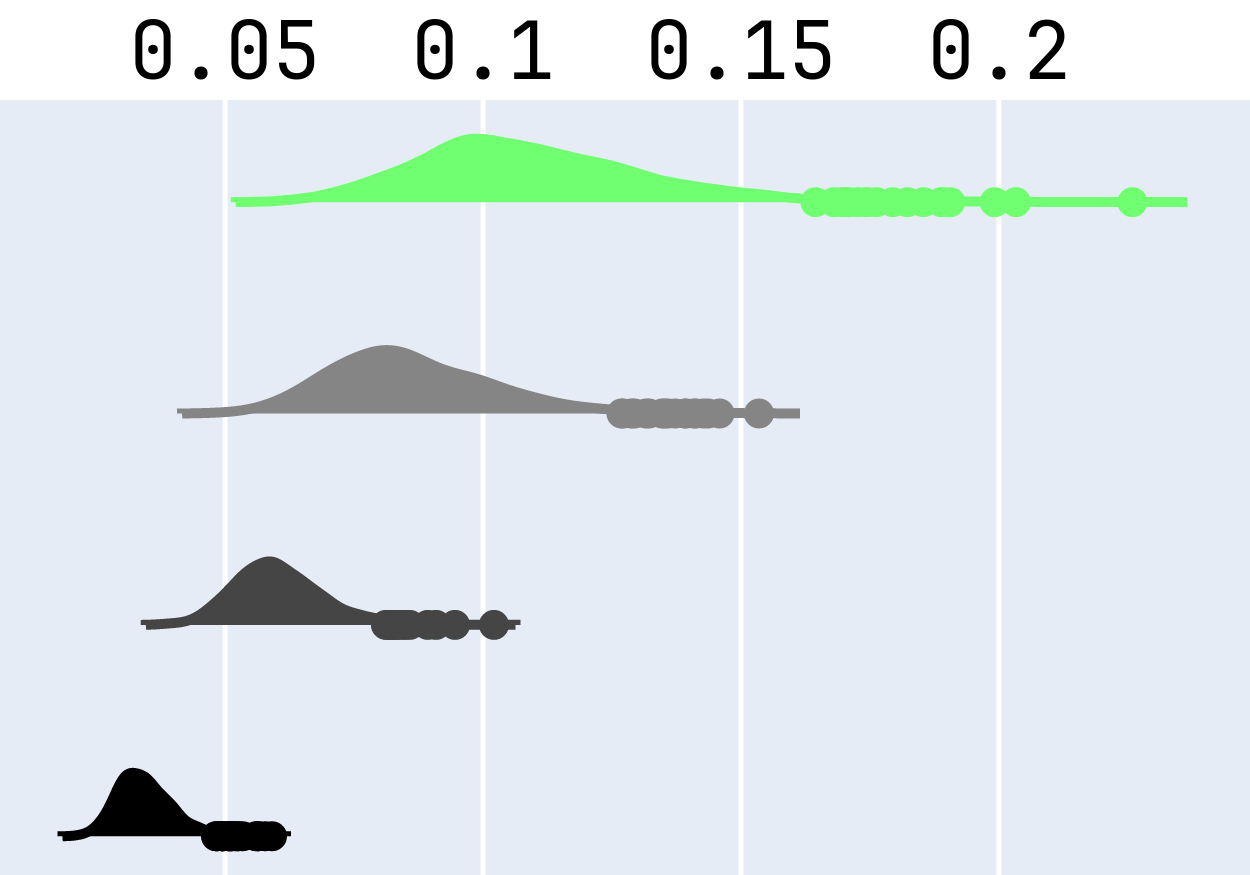
\includegraphics[width=\linewidth]{images/npsk_MSS_0.png}
      \end{minipage}
      \hspace{0.015\textwidth}%
      \begin{minipage}[t]{0.31\textwidth}
        \centering
        \normalsize\bfseries P-Loss\\[0.3em]
        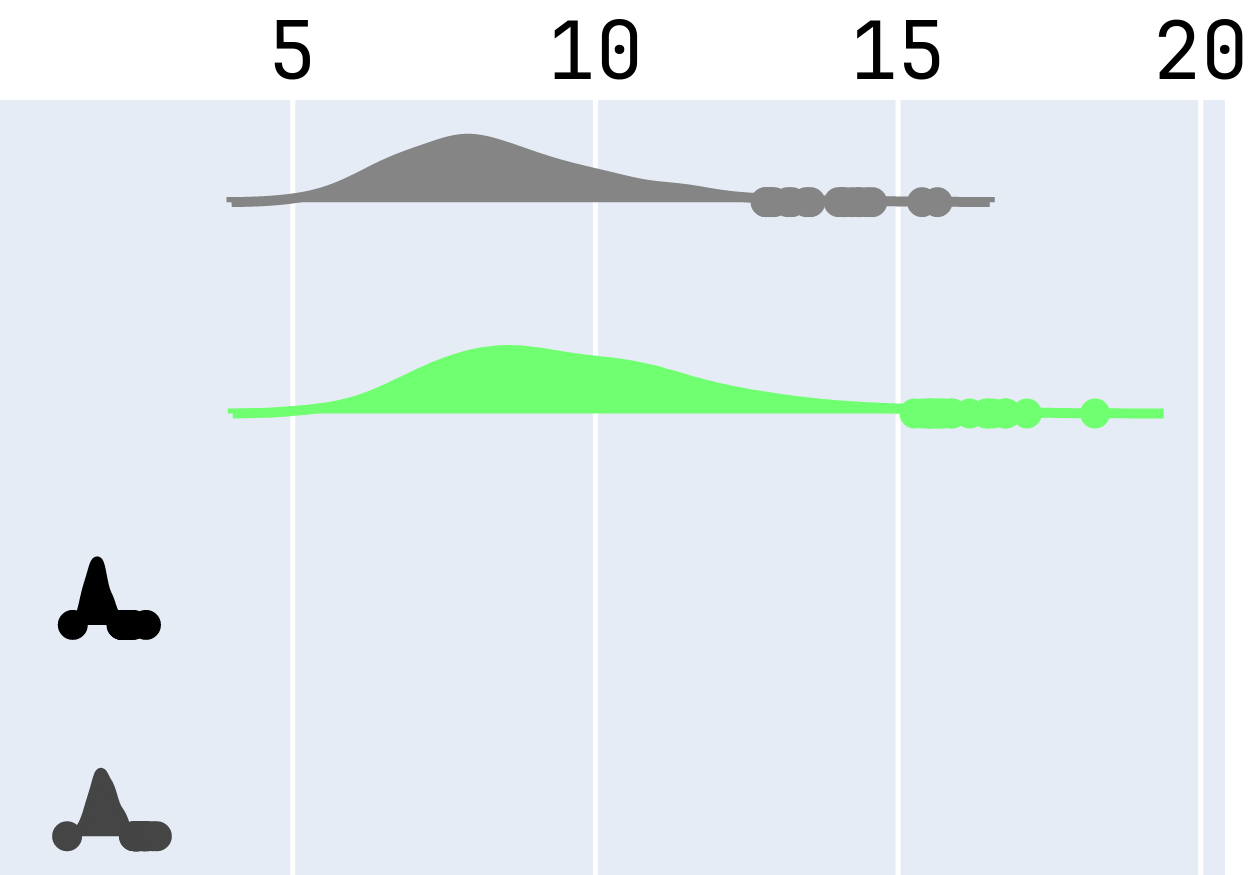
\includegraphics[width=\linewidth]{images/npsk_P-Loss_0.png}
      \end{minipage}
      \hspace{0.01\textwidth}%
      \begin{minipage}[t]{0.31\textwidth}
        \centering
        \normalsize\bfseries Likert\\[0.3em]
        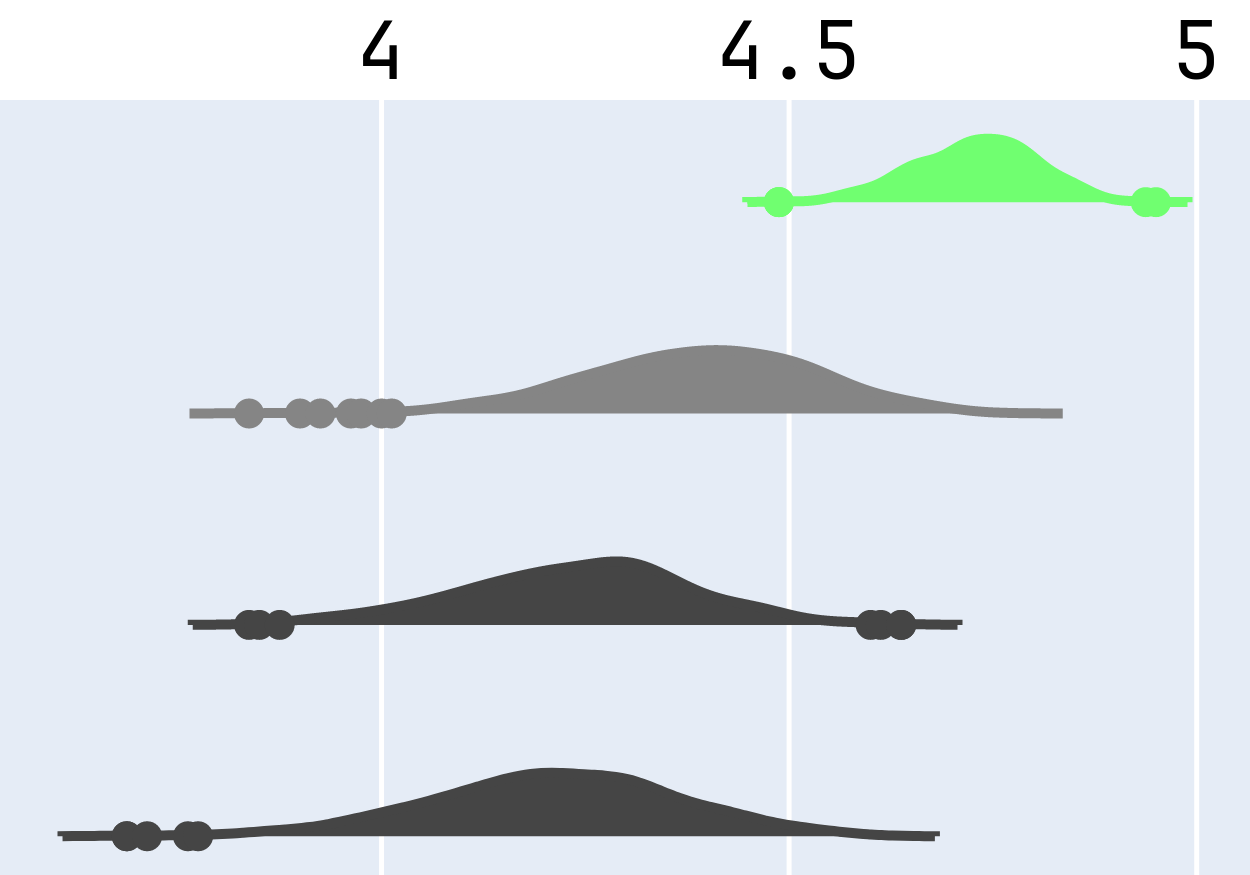
\includegraphics[width=\linewidth]{images/npsk_likert_0.png}
      \end{minipage}
    \end{minipage}
  \end{minipage}
  \label{fig:npsk_p0}
}\\[0.5em]

% 2nd row
\subfloat[\AddSineSaw~bootstrapped distributions and ranks given by NPSK.]{
  \begin{minipage}{\textwidth}
    \begin{minipage}{0.03\textwidth}
      \footnotesize\raggedleft
      \vspace{0.5cm}
      SIMSE\\[0.6cm]
      L1\\[0.65cm]
      JTFS\\[0.65cm]
      DTW
    \end{minipage}%
    \begin{minipage}{0.98\textwidth}\centering
      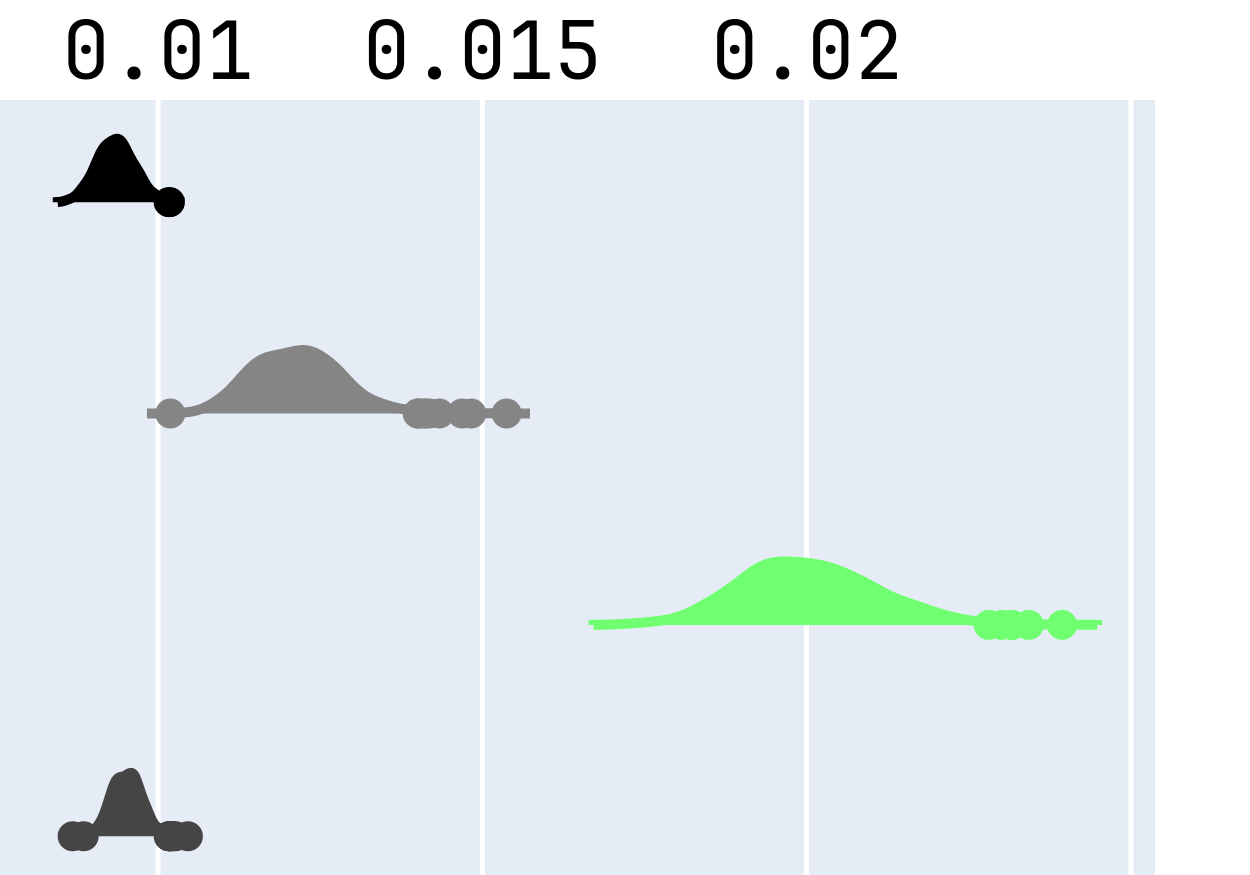
\includegraphics[width=0.31\textwidth]{images/npsk_MSS_1.png}%
      \hspace{0.015\textwidth}%
      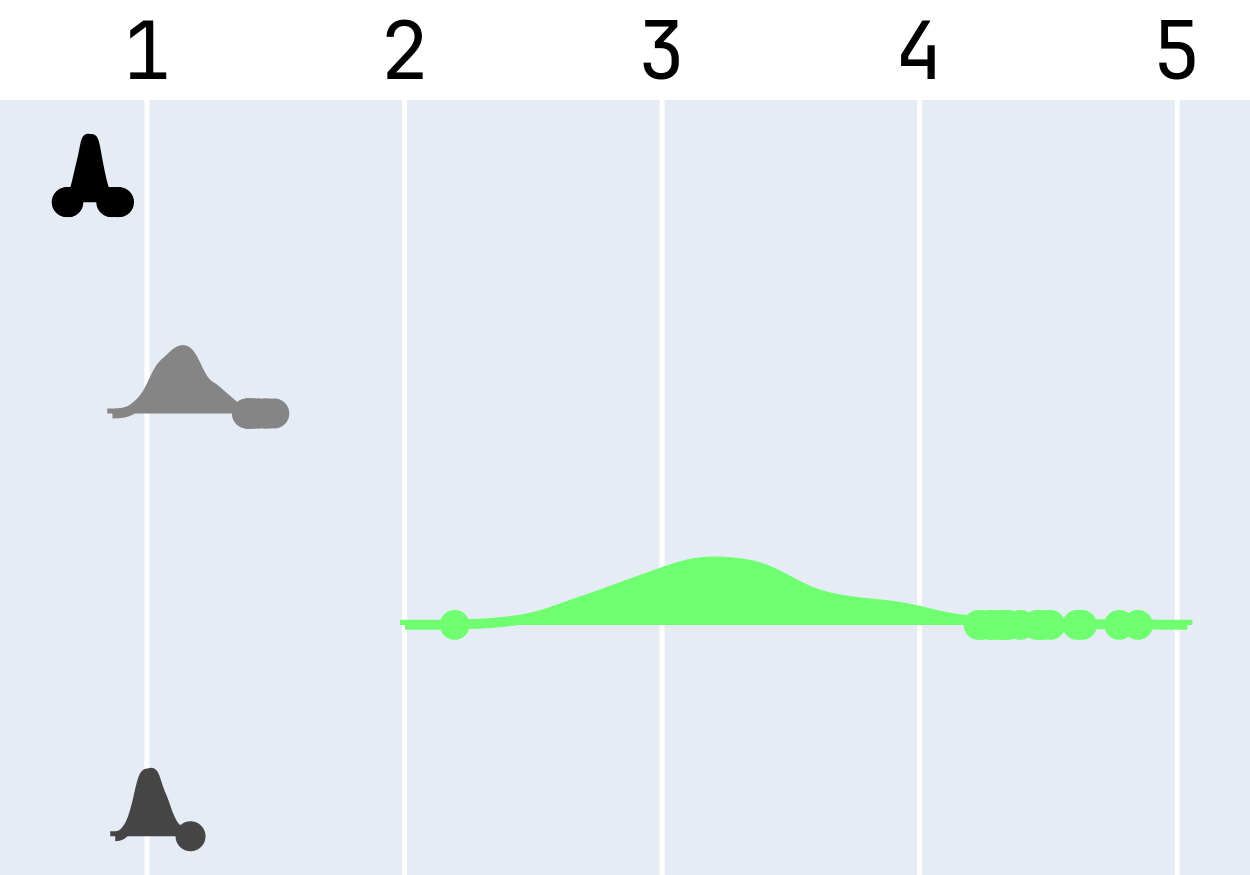
\includegraphics[width=0.31\textwidth]{images/npsk_P-Loss_1.png}%
      \hspace{0.015\textwidth}%
      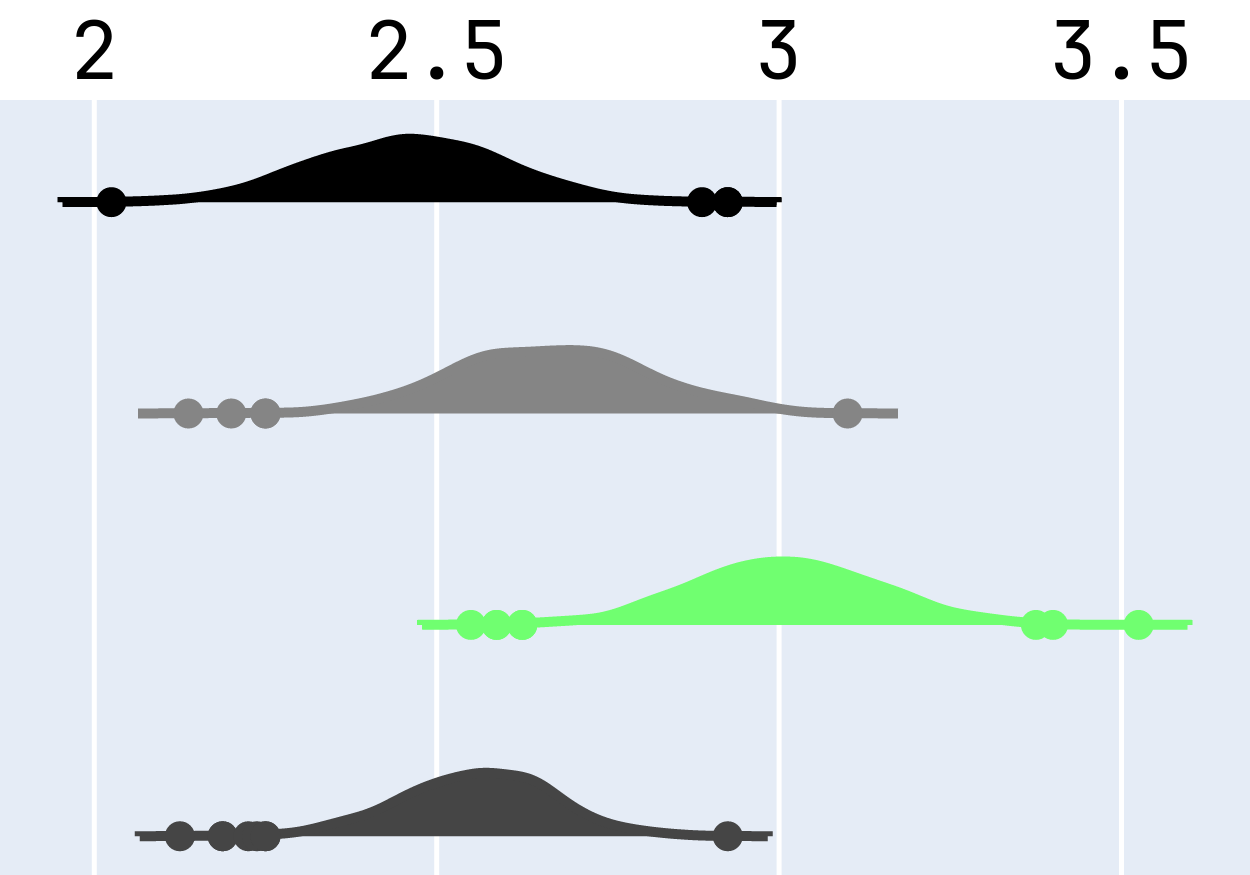
\includegraphics[width=0.31\textwidth]{images/npsk_likert_1.png}
    \end{minipage}
  \end{minipage}
  \label{fig:npsk_p1}
}\\[0.5em]

% 3rd row
\subfloat[\AmpMod~bootstrapped distributions and ranks given by NPSK.]{
  \begin{minipage}{\textwidth}
    \begin{minipage}{0.03\textwidth}
      \footnotesize\raggedleft
      \vspace{0.5cm}
      SIMSE\\[0.6cm]
      L1\\[0.65cm]
      JTFS\\[0.65cm]
      DTW
    \end{minipage}%
    \begin{minipage}{0.98\textwidth}\centering
      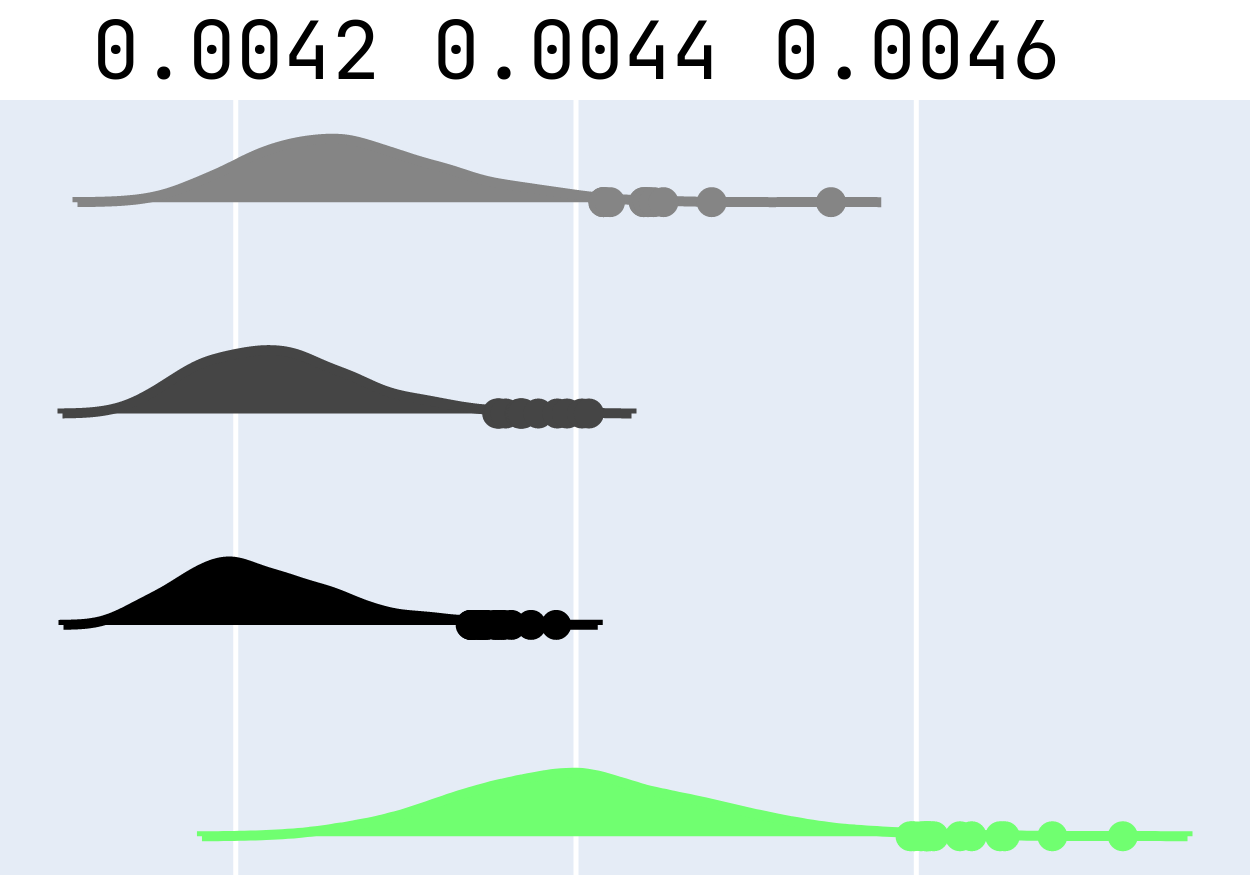
\includegraphics[width=0.31\textwidth]{images/npsk_MSS_2.png}%
      \hspace{0.015\textwidth}%
      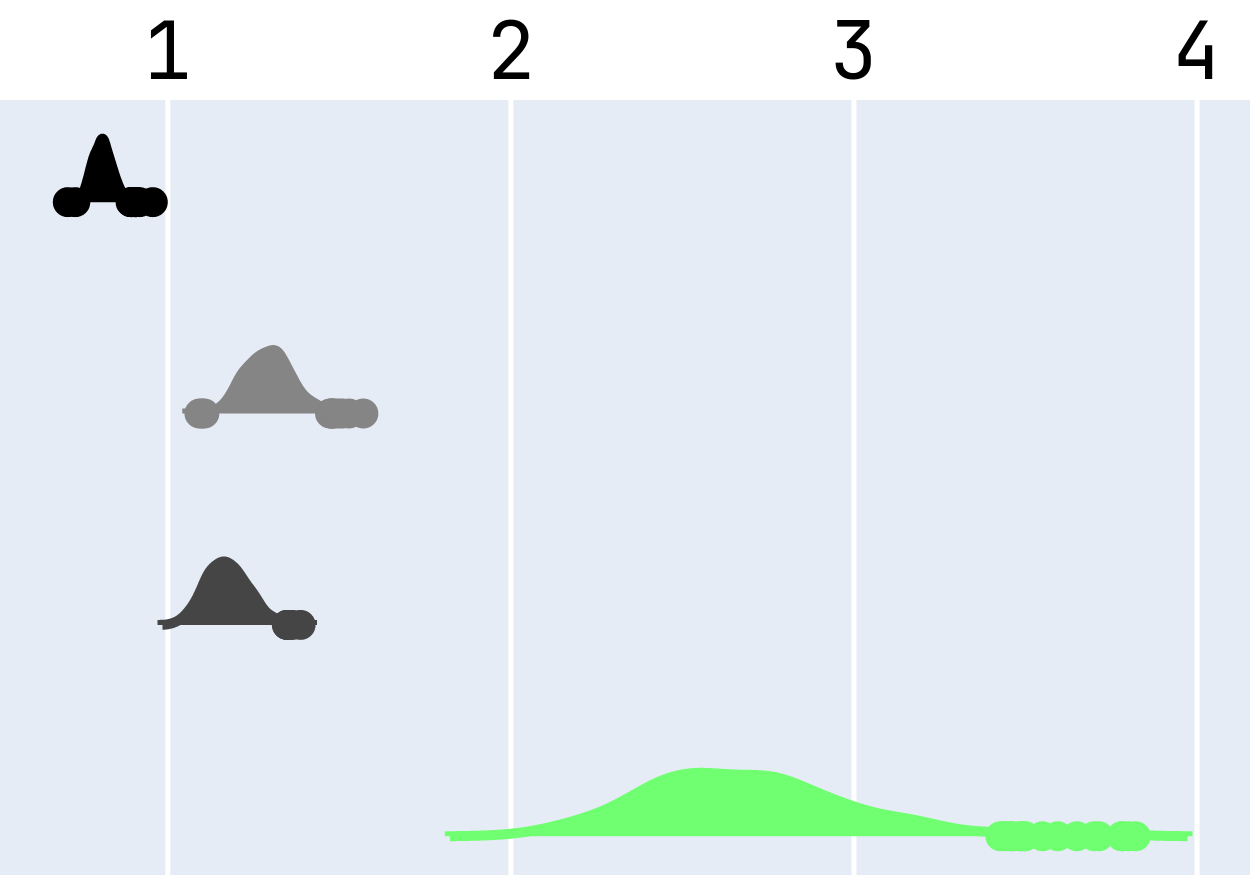
\includegraphics[width=0.31\textwidth]{images/npsk_P-Loss_2.png}%
      \hspace{0.015\textwidth}%
      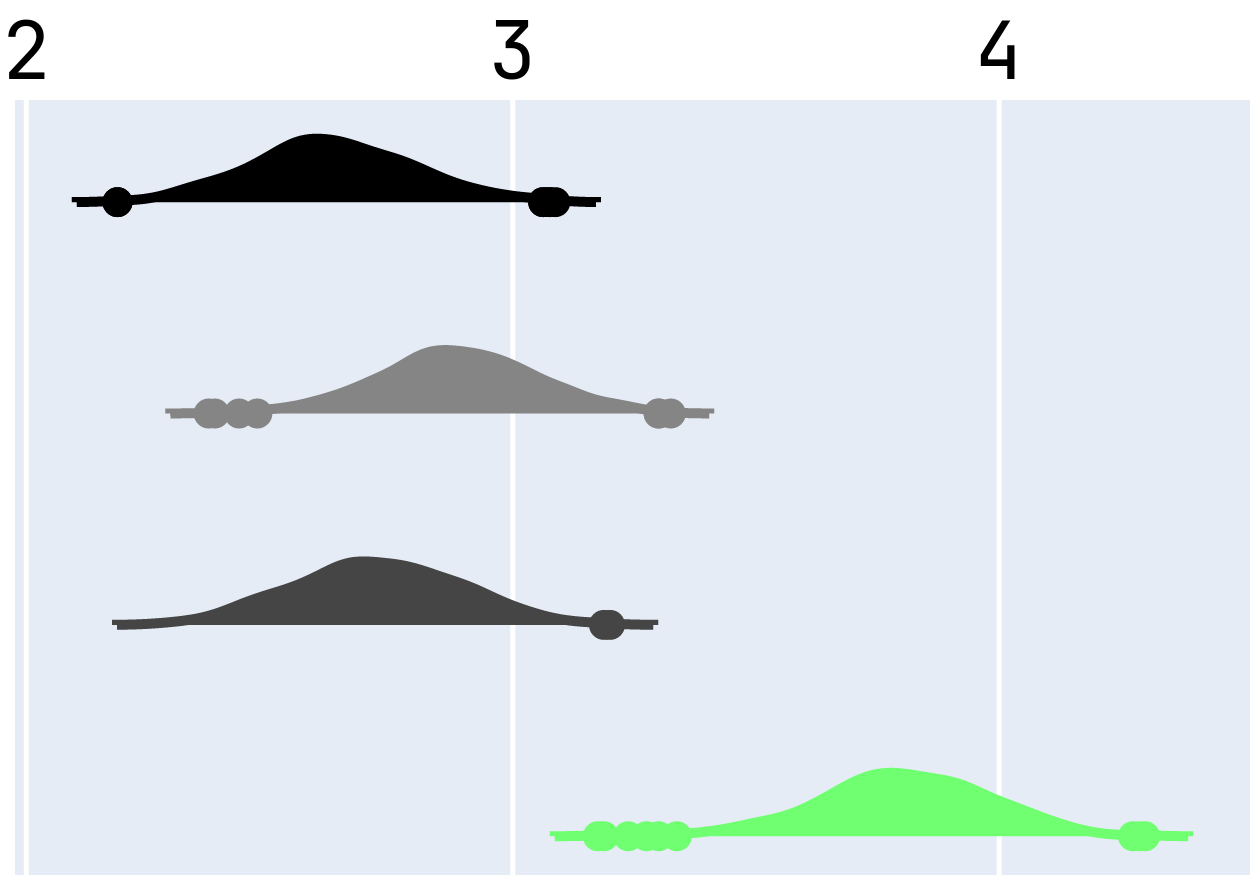
\includegraphics[width=0.31\textwidth]{images/npsk_likert_2.png}
    \end{minipage}
  \end{minipage}
  \label{fig:npsk_p2}
}\\[0.5em]

% 4th row
\subfloat[\FMMod~bootstrapped distributions and ranks given by NPSK.]{
  \begin{minipage}{\textwidth}
    \begin{minipage}{0.03\textwidth}
      \footnotesize\raggedleft
      \vspace{0.5cm}
      SIMSE\\[0.6cm]
      L1\\[0.65cm]
      JTFS\\[0.65cm]
      DTW
    \end{minipage}%
    \begin{minipage}{0.98\textwidth}\centering
      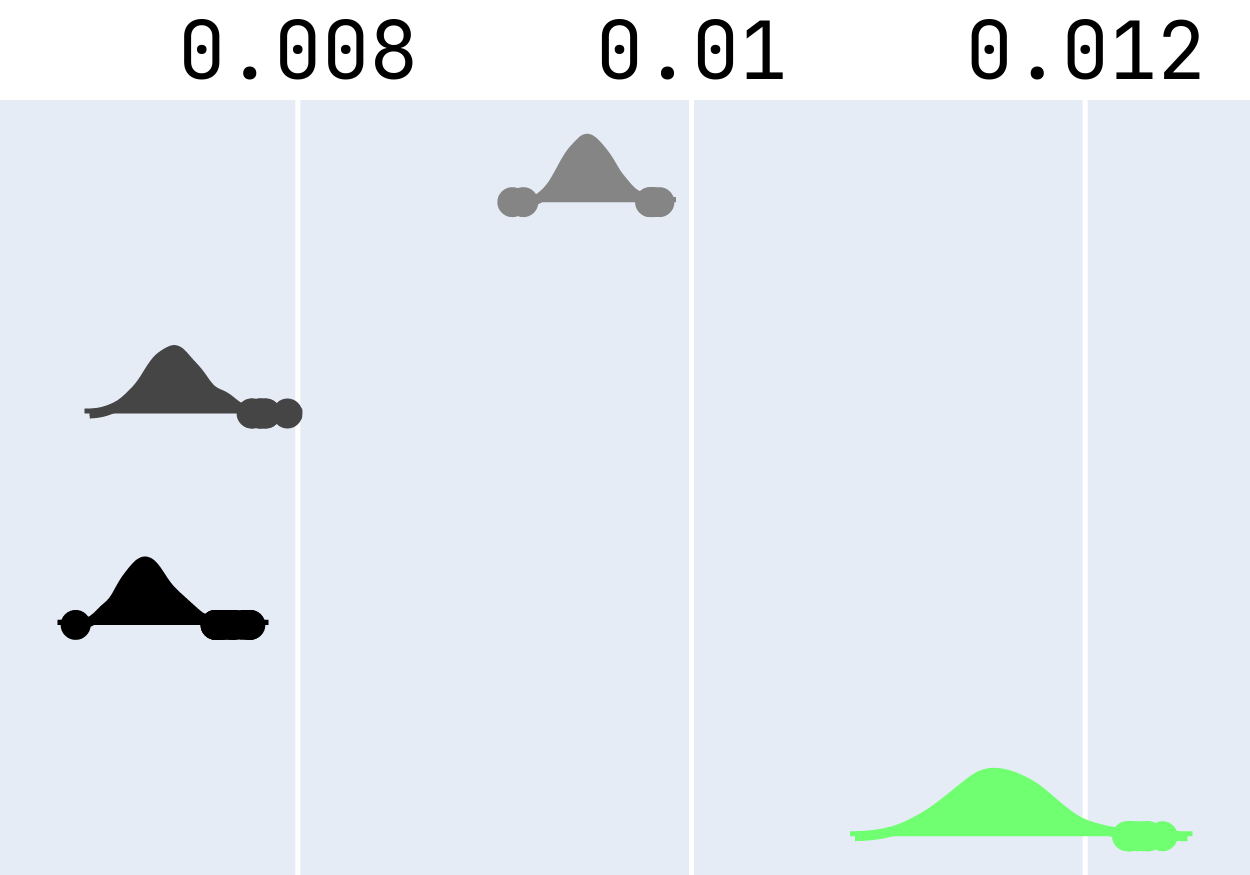
\includegraphics[width=0.31\textwidth]{images/npsk_MSS_3.png}%
      \hspace{0.015\textwidth}%
      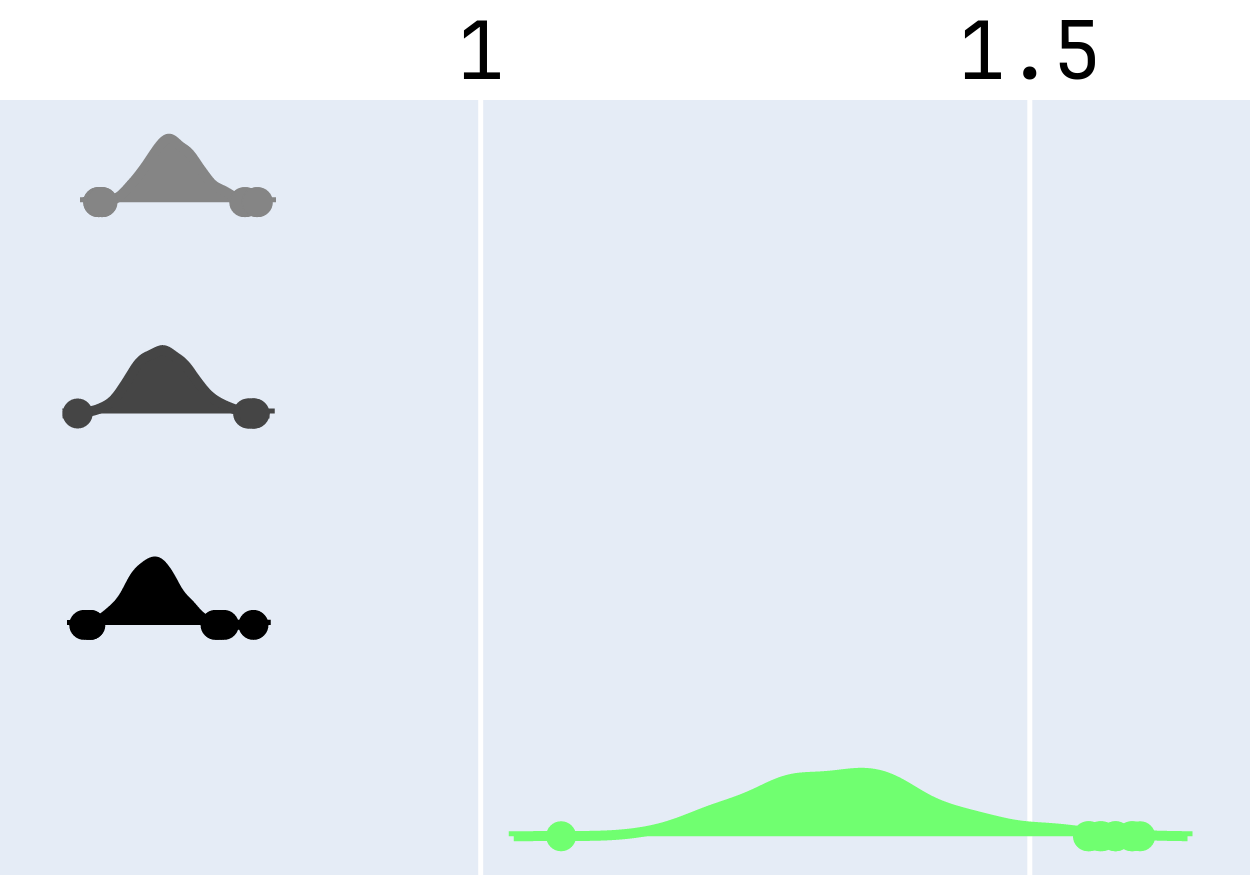
\includegraphics[width=0.31\textwidth]{images/npsk_P-Loss_3.png}%
      \hspace{0.015\textwidth}%
      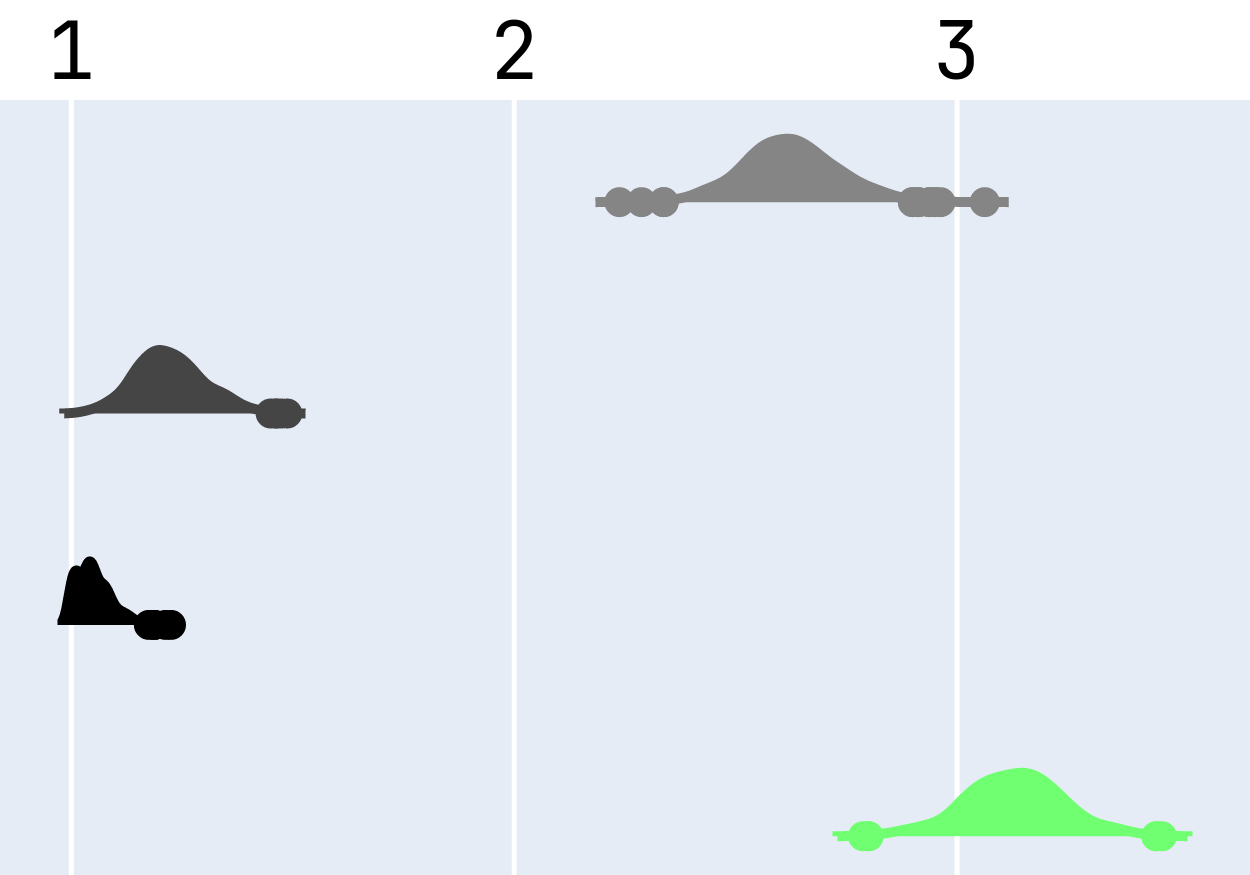
\includegraphics[width=0.31\textwidth]{images/npsk_likert_3.png}
    \end{minipage}
  \end{minipage}
  \label{fig:npsk_p3}
}

\caption{Distributions and ranks of the loss functions based on three different performance measures. From left to right, the performance measures are: MSS, P-Loss, and Likert. Higher values indicate better performance. Rank colors are \colorbox{rank1}{\textcolor{black}{\textbf{1}}} \colorbox{rank2}{\textcolor{white}{\textbf{2}}} \colorbox{rank3}{\textcolor{white}{\textbf{3}}} \colorbox{rank4}{\textcolor{white}{\textbf{4}}}.}
\label{fig:npsk_all}
\end{figure*}


\subsubsection{\BPNoise}
For this synthesizer program, the spectrogram-based models performed the best. This makes intuitive sense, as the visual effects of a band-pass filter on white noise are readily apparent in a spectrogram. As shown in Figure~\ref{fig:npsk_p0}, manual hearing test and MSS selected \SIMSESpec~as the best performer and \LoneSpec~as the second-best performer, while P-Loss gave the reverse order. 


\subsubsection{\AddSineSaw}
As shown in Figure~\ref{fig:npsk_p1}, JTFS was the best performing loss function in all evaluation methods. Moreover, all evaluation methods produced identical results. 

\subsubsection{\AmpMod}
IP-Loss and manual hearing tests yield identical rankings, and MSS results vary for for ranks 2 to 4. It is not surprising that MSS results differ from the hearing tests, as we saw in Table~\ref{tab:kruskal_auto}, MSS showed no significant differences between groups. As shown in Figure~\ref{fig:npsk_p2}, all models selected \DTWEnv~as the best performer. This may be due to \DTWEnv's focus on periodic changes in loudness.

\subsubsection{\FMMod}
\DTWEnv~is again the best performer here. As shown in Figure~\ref{fig:npsk_p3}, all methods of analysis gave identical rankings to all programs.

\subsection{Consistency In Rankings}
\label{sec:consistency_in_rankings}
\subsubsection{Manual Ranks} Agreement between the manually assigned scores is measured using Spearman’s rank correlation, which provides both a correlation coefficient ($\rho$) ranging from –1 (perfect negative correlation) to 1 (perfect positive correlation), and a p-value testing the null hypothesis of no correlation~\cite{spearman1987proof,rebekic2015pearson}. Across all programs, the correlation was very strong ($\rho = 0.86$, $p < 10^{-180}$). Per-program correlations were also very strong: $\rho = 0.71$ for \BPNoise{} ($p < 10^{-25}$), $\rho = 0.64$ for \AddSineSaw{} ($p < 10^{-19}$), $\rho = 0.84$ for \AmpMod{} ($p < 10^{-43}$), and $\rho = 0.85$ for \FMMod{} ($p < 10^{-44}$). 

Table~\ref{tab:combined_ranks} shows the SNPK rankings of bootstrapped evaluation results for each program. Both MSS and P-Loss gave a different rank from the hearing results in 3 out of 16 cases, which shows consistency between automatic and manual hearing tests, at least for the simple programs used in this work. We also observe that top ranks were consistent across performance evaluation methodologies, with the exception of P-Loss in \BPNoise, which narrowly picks a different spectrogram-based loss function.
% \noindent\textit{Ranks that differ from the hearing test are marked with an asterisk.}

\begin{table}[htbp]
\centering
\begin{minipage}{0.45\textwidth}
    \centering
    \begin{tabular}{|c|c|c|c|}
    \hline
    \textbf{Function} & \textbf{MSS} & \textbf{P-LOSS} & \textbf{Hearing} \\
    \hline
    \textbf{SIMSE} & 1\phantom{*} & 2* & 1\phantom{*} \\
    \textbf{L1}    & 2\phantom{*} & 1* & 2\phantom{*} \\
    \textbf{JTFS}  & 3\phantom{*} & 4* & 3\phantom{*} \\
    \textbf{DTW}   & 4*           & 3\phantom{*} & 3\phantom{*} \\
    \hline
    \end{tabular}
    \caption{\footnotesize \BPNoise~ranks}
    \label{tab:p0}
\end{minipage}%
\hspace{1cm}
\begin{minipage}{0.45\textwidth}
    \centering
    \begin{tabular}{|c|c|c|c|}
    \hline
    \textbf{Function}& \textbf{MSS} & \textbf{P-LOSS} & \textbf{Hearing} \\
    \hline
    \textbf{SIMSE} & 4\phantom{*} & 4\phantom{*} & 4\phantom{*} \\
    \textbf{L1} & 2\phantom{*} & 2\phantom{*} & 2\phantom{*} \\
    \textbf{JTFS} & 1\phantom{*} & 1\phantom{*} & 1\phantom{*} \\
    \textbf{DTW} & 3\phantom{*} & 3\phantom{*} & 3\phantom{*} \\
    \hline
    \end{tabular}
    \caption{\footnotesize \AddSineSaw~ranks}
    \label{tab:p1}
\end{minipage}

\vspace{0.5cm} % Adds vertical space between rows of tables

\begin{minipage}{0.45\textwidth}
    \centering
    \begin{tabular}{|c|c|c|c|}
    \hline
    \textbf{Function} & \textbf{MSS} & \textbf{P-LOSS} & \textbf{Hearing} \\
    \hline
    \textbf{SIMSE} & 3* & 4\phantom{*} & 4\phantom{*} \\
    \textbf{L1}    & 2\phantom{*} & 2\phantom{*} & 2\phantom{*} \\
    \textbf{JTFS}  & 4* & 3\phantom{*} & 3\phantom{*} \\
    \textbf{DTW}   & 1\phantom{*} & 1\phantom{*} & 1\phantom{*} \\
    \hline
    \end{tabular}
    \caption{\footnotesize \AmpMod~ranks}
    \label{tab:p2}
\end{minipage}%
\hspace{1cm}
\begin{minipage}{0.45\textwidth}
    \centering
    \begin{tabular}{|c|c|c|c|}
    \hline
    \textbf{Function} & \textbf{MSS} & \textbf{P-LOSS} & \textbf{Hearing} \\
    \hline
   \textbf{SIMSE} & 2\phantom{*} & 2\phantom{*} & 2\phantom{*} \\
    \textbf{L1} & 3\phantom{*} & 3\phantom{*} & 3\phantom{*} \\
    \textbf{JTFS} & 4\phantom{*} & 4\phantom{*} & 4\phantom{*} \\
    \textbf{DTW} & 1\phantom{*} & 1\phantom{*} & 1\phantom{*} \\
    \hline
    \end{tabular}
    \caption{\footnotesize \FMMod~ranks}
    \label{tab:p3}
\end{minipage}
\end{table}





\section{Takeaways, Practical Implications, and Caveats}
% (Q1) To what extent do automatic evaluation metrics agree with manual listening tests? (Q2) Can novel loss functions utilizing Dynamic Time Warping (DTW) and Scale-Invariant Mean Squared Error (SIMSE) provide advantages over standard loss functions, and if so, when? (Q3) Is an iterative differentiable optimization a viable strategy for design of sound-matching experiments?
The experiment results provide answers regarding the main hypothesis of this work as well as the secondary questions. Based on these answers, we can make practical recommendations for future research. 

\subsection{Takeaways}
Perhaps the most important takeaway regarding our main hypothesis is that the loss function that yields the best sound-matching outcomes varies depending on the synthesizer program. This is likely due to the interaction between how the parameters of the synthesizer influence the sound, and the core sonic features used by the loss function.

\textbf{Q1}: To what extent do automatic evaluation metrics agree with manual listening tests? we see somewhat consistent results between the rankings assigned by manual hearing tests (which we take as the ground truth), and automatic measures of P-Loss and MSS. With the exception of P-Loss in \BPNoise{} narrowly selecting a different spectrogram based loss, all measures of performance selected the same top performer. Due to the simplicity of our programs and the occasional deviations, we cannot conclude that these automatic measures are substitutes for human hearing tests. As many previous works have done\todo{cite}, the use of MSS and/or P-Loss as general loss functions does seem appropriate, however, we advise the use of listening tests or custom made loss functions for more specific analysis. 

\textbf{Q2}: Are DTW and SIMSE effective measures of loss? If so, 

 \DTWEnv{} consistently outperformed other measures in amplitude-modulated synthesis, where envelope alignment is critical. \SIMSESpec{} performed best in subtractive synthesis, where scale-invariance captures noise filtering effects more robustly than L1-based measures. These results indicate that the advantages of novel losses are context-dependent, and the necessity of further creative approaches to differentiable sound-similarity measures. 

\textbf{Q3}: Can iterative differentiable optimization be applied effectively in synthesizers using classical DSP functions?
The approach of designing DSP functions in Faust and transpiling to differentiable Faust code yielded meaningful outputs and enabled comparative evaluation of losses. The use of Faust for synthesizer definition was convenient, and transpiling to Jax enabled quick gradient optimization. We were able to run our 1200 experiments within 72 hours on a laptop without a GPU\footnote{Lenovo ThinkPad T480, i5-8350U CPU at 1.70GHz, 32 GB RAM.}.

\subsection{Practical Recommendations:}
Based on our findings, several actionable guidelines emerge. These heuristics can guide practitioners in selecting appropriate similarity measures and synthesis methods for future sound-matching experiments.
\begin{itemize}
    \item In leu of listening tests, MSS or P-Loss are generally useful for large-scale benchmarking, but confirm conclusions with manual listening when accuracy in isolated cases is important. 
    \item For amplitude-modulated synthesis, DTW-based losses (e.g., \DTWEnv{}) are most effective.
    \item For subtractive/noise-filtered synthesis, spectrogram based losses are most effective. We can recommend the use of SIMSE over L1, particularly when relative amplitudes are less important. 
    \item Iterative differentiable optimization via Faust-to-JAX is a viable strategy for defining various differentiable DSP functions, requiring only modest hardware resources.
\end{itemize}

\subsection{Applicability to More Complex Synthesizers}
The experiments in this study were conducted with differentiable synthesizers of modest complexity (2 parameters each), chosen to isolate fundamental synthesis principles. 
While this level of simplicity facilitates controlled comparisons, it does not fully capture the parameter richness of real-world synthesizers, which can have hundreds of parameters routed in various ways. The generalizability of our findings does require further research.

Nonetheless, we believe that the insights here can extend naturally to more complex domains. First, the observed dependence of loss performance on synthesis method is will likely remain stable even with added complexities such as layers of modulation, filtering, or nonlinearity. \DTWEnv{} and \SIMSESpec{} measure very specific features of audio, and their use in the recommended settings would likely yield the desired results regardless of synthesizer complexity. 

(same as previous sentence) Second, the heuristics identified here (e.g., DTW\_Envelope excelling in amplitude-modulated contexts, SIMSE\_Spec in subtractive filtering) map directly onto common building blocks found in commercial and modular synthesizers, suggesting that these recommendations can guide loss selection in practical scenarios.

% Third, the iterative differentiable optimization framework proved viable even on limited hardware, which indicates that similar pipelines could be applied to larger differentiable synthesizers if computational resources allow.

% At the same time, real-world synthesizers present new challenges. 
% High-dimensional parameter spaces may exacerbate issues of local minima and make optimization less stable, particularly when loss functions are only partially informative. 


% Non-differentiable components (e.g., physical modeling, complex routing) also limit the direct applicability of gradient-based methods. 

% Future work should therefore investigate hybrid approaches, combining differentiable blocks with surrogate models or gradient-free optimization for non-differentiable components. 
% Out-of-domain targets, such as recorded instruments or environmental sounds, represent another direction where the loss–synth interaction may behave differently than in controlled in-domain experiments.
